\documentclass[10pt,xcolor=pdflatex]{beamer}
\usepackage{newcent}
\usepackage[utf8]{inputenc}
%\usepackage[czech]{babel}
\usepackage{hyperref}
\usepackage{fancyvrb}
\usepackage{graphicx}
\graphicspath{ {./img/} }
\usetheme{FIT}

%%%%%%%%%%%%%%%%%%%%%%%%%%%%%%%%%%%%%%%%%%%%%%%%%%%%%%%%%%%%%%%%%%
\title[Generátor veděckých portálů]{Generátor veděckých portálů}

\author[Jiří Furda]{Jiří Furda\\*Doc. RNDr. Pavel Smrž, Ph.D.}

\institute[FIT VUT]{Fakulta informačních technologií Vysokého učení technického v Brně\\
Bo\v{z}et\v{e}chova 1/2. 612 66 Brno - Kr\'alovo Pole\\
xfurda00@stud.fit.vutbr.cz}

\date{29. ledna 2019}
%\date{\today}
%\date{} % bez data

%%%%%%%%%%%%%%%%%%%%%%%%%%%%%%%%%%%%%%%%%%%%%%%%%%%%%%%%%%%%%%%%%%

\begin{document}

\frame[plain]{\titlepage}

\begin{frame}
    \frametitle{Motivace}
    \begin{center}
        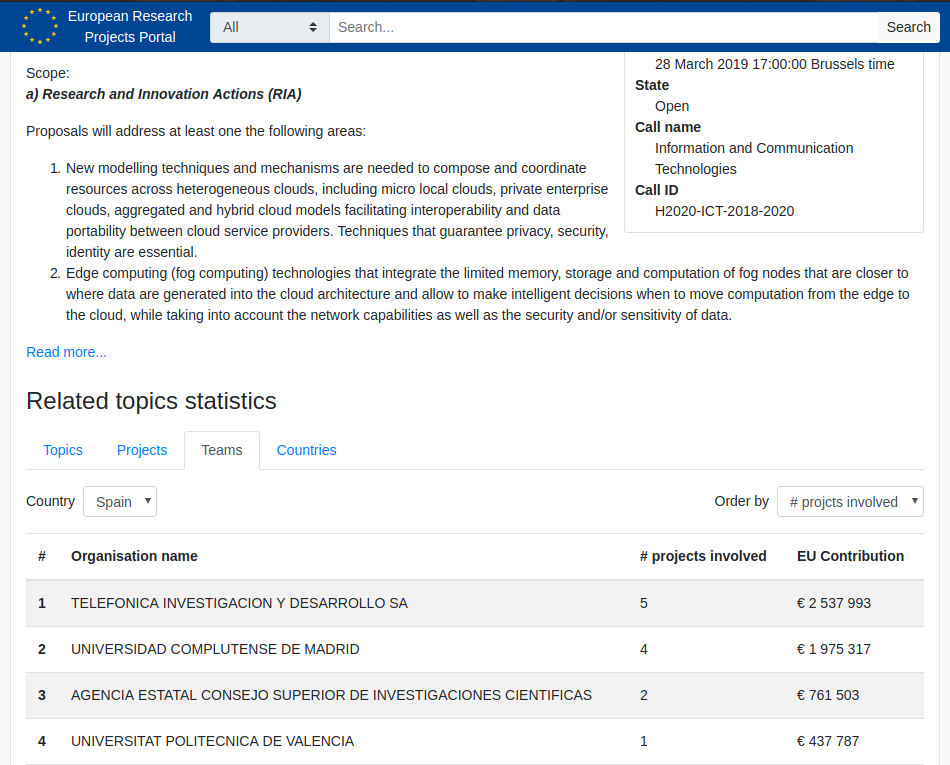
\includegraphics[scale=0.29]{img/teams_statistic.png}
    \end{center}
\end{frame}

    
\begin{frame}
    \frametitle{Cíle práce}
    \begin{itemize}
        \item Technologická aktualizace původního portálu
            \begin{itemize}
                \item Přechod z \emph{ElasticUtils} na \emph{Elasticsearch DSL}
                \item Nové uživatelské rozhraní
                \item Refaktorizace
        	\end{itemize}
    	\item Rozšíření poskytovaného obsahu
    	    \begin{itemize}
                \item Začlenění obsahu výzev
                \item Provazování výzev s předchozími tématy projektů
                \item Vyhledávání stránek týmů a osob
                \item Indexování celého obsahu webových stránek projektů
        	\end{itemize}
        \item Zlepšení vyhledávání a extrakce stránek projektů a odevzdávaných zpráv z nich
    	\item Nový zdroj získávání dat
    	    \begin{itemize}
                \item \emph{Participant Portal} bude nahrazen \emph{Funding and Tenders Portal}
        	\end{itemize}    	    
	\end{itemize}
\end{frame}


\begin{frame}
    \frametitle{Současný stav}
    
    \begin{itemize}
        \item \emph{Webový portál}
        \begin{itemize}
            \item Refaktorizace (50\%)
            \item Uživatelské rozhraní (65\%)
	    \end{itemize}    
	    
	   \item \emph{Extraktor dat}
        \begin{itemize}
            \item Začlenění výzev (50\%)
            \item Nový zdroj dat (10\%)
            \item Stránky týmů a osob (0\%)
            \item Indexace stránek projektů (0\%)
	    \end{itemize}    
	\end{itemize}    
\end{frame}


\begin{frame}
    \frametitle{Výsledky v 1. semestru}
    
    \begin{itemize}
        \item Portál beží na \emph{Elasticsearch 6.4}
        \item Uživatelské rozhraní lépe pracuje s prostorem
        \item Portál umožňuje \emph{vyhledat výzvy}
        \item Portál \emph{propojuje podobné výzvy}
    \end{itemize}    
\end{frame}


\begin{frame}
    \frametitle{Vyhodnocení a zjištěné nedostatky}
    
    \begin{itemize}
        \item Získání znalosti použití jazyku \emph{Python pro webové aplikace}
        \item Získání znalosti práce s Elasticsearch
        \item Náhled do problematiky \emph{web scrapingu}
        
        \item Problémy
        \begin{itemize}
            \item Počáteční bariéra s použitými technologiemi a kódem
            \item Nedostatek času v průběhu semestru
        \end{itemize} 
        
    \end{itemize}    
\end{frame}


\begin{frame}
    \frametitle{Plán na letní semestr}
    \begin{enumerate}
        \item Zlepšení struktury kódu (do \emph{17. 2.})
        \item Implementace chybějící funkcionality portálu (do \emph{3. 3.})
        \item Doladění uživatelského rozhraní (do \emph{10. 3.})
        \item Napojení na Funding and Tenders Portal (do \emph{17. 3.})
        \item Vyhledávání stránek týmů, osob a projektů (do \emph{31. 3.})
        \item Sepsání bakalářské práce (do \emph{30. 4.})
    \end{enumerate}
\end{frame}


\bluepage{Děkuji za pozornost!}

\end{document}

